\documentclass[aspectratio=169,10pt]{beamer}
\usetheme{metropolis}
\usepackage{amsmath,amssymb,bm}
\usepackage{siunitx}
\usepackage{booktabs}
\usepackage{tikz}
\usetikzlibrary{arrows.meta,calc,positioning,patterns}
\usepackage{pgfplots}
\pgfplotsset{compat=1.17}
\sisetup{per-mode=symbol,detect-all}
\metroset{numbering=fraction,progressbar=frametitle,block=fill}
\tikzset{capt/.style={text width=5.2cm,align=center}}
\hypersetup{colorlinks=true,urlcolor=blue!60!black,linkcolor=.}
% ITU logo on every frame (top-right): white on the dark title bar, navy on the title page.
\addtobeamertemplate{frametitle}{}{%
  \begin{tikzpicture}[remember picture,overlay]
    \node[anchor=north east,yshift=-1.5pt,xshift=-6pt] at (current page.north east) {
\includegraphics[height=0.7cm]{logos/itu_logo_beyaz.pdf}};
  \end{tikzpicture}}
\titlegraphic{\hfill
\includegraphics[height=1.6cm]{logos/itu_logo_laci.pdf}}

\title{Lecture 4: Fatigue under Combined and Variable Loading}
\subtitle{UCK 364E Design of Machine Elements}
\author{Prof.\ Dr.\ Onur Tunçer}
\institute{Department of Aeronautical Engineering, Istanbul Technical University}
\date{Fall 2026}

\begin{document}
\maketitle

\begin{frame}{Today}
\begin{enumerate}
  \item Why uniaxial fatigue is not enough
  \item Proportional and non-proportional loading
  \item The von Mises amplitude and the DE--Goodman shaft equation
  \item The Gough ellipse
  \item Critical-plane methods --- what they are and when you need them
  \item Rainflow counting: why, and how to do it by hand
  \item Miner on a counted spectrum
  \item Where an aircraft spectrum comes from
  \item Scatter and the design S--N curve
\end{enumerate}
\end{frame}


\begin{frame}{The road map: what we are actually computing}
\centering

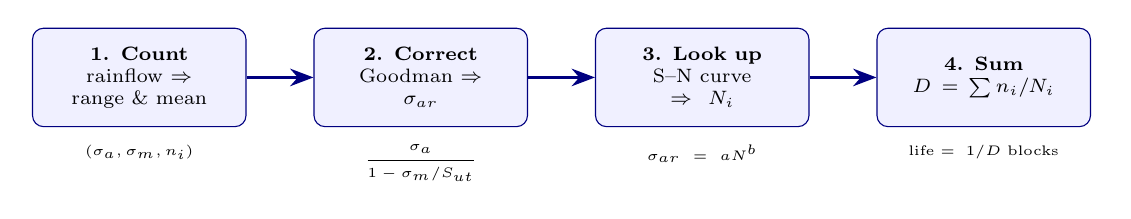
\begin{tikzpicture}[scale=1.0,>=Stealth,font=\scriptsize,
  box/.style={draw=blue!50!black,fill=blue!6,rounded corners,align=center,minimum height=1.25cm,text width=2.5cm,inner sep=3pt}]
\node[box] (a) {\textbf{1. Count}\\ rainflow $\Rightarrow$\\ range \& mean};
\node[box,right=0.85cm of a] (b) {\textbf{2. Correct}\\ Goodman $\Rightarrow$\\ $\sigma_{ar}$};
\node[box,right=0.85cm of b] (c) {\textbf{3. Look up}\\ S--N curve\\ $\Rightarrow N_i$};
\node[box,right=0.85cm of c] (d) {\textbf{4. Sum}\\ $D=\sum n_i/N_i$};
\foreach \x/\y in {a/b,b/c,c/d} \draw[->,very thick,blue!50!black] (\x) -- (\y);
\node[font=\tiny,anchor=north,text width=2.6cm,align=center] at ($(a.south)+(0,-0.1)$) {$(\sigma_a,\sigma_m,n_i)$};
\node[font=\tiny,anchor=north,text width=2.6cm,align=center] at ($(b.south)+(0,-0.1)$) {$\dfrac{\sigma_a}{1-\sigma_m/S_{ut}}$};
\node[font=\tiny,anchor=north,text width=2.6cm,align=center] at ($(c.south)+(0,-0.1)$) {$\sigma_{ar}=aN^{b}$};
\node[font=\tiny,anchor=north,text width=2.8cm,align=center] at ($(d.south)+(0,-0.1)$) {life $=1/D$ blocks};
\end{tikzpicture}

\vspace{6pt}

\raggedright
Everything in this lecture is one of these four boxes.
\begin{itemize}\footnotesize
  \item \alert{Box 1} is new today (rainflow) --- and it is where the multiaxial problem also lands, because you must reduce the stress \emph{state} to one number before you can count it
  \item \alert{Boxes 2 and 3} you already know from Lecture 2
  \item \alert{Box 4} is a sum --- the easy part, and the part with all the caveats
\end{itemize}
\end{frame}

\section{Why this lecture exists}

\begin{frame}{Almost nothing is loaded uniaxially}
\footnotesize
\begin{tabular}{@{}lll@{}}
\toprule
Element & Stress state & Phasing \\
\midrule
Rotating shaft with a pulley & bending (alternating) $+$ torsion (steady) & fixed ratio \\
Landing-gear axle & bending from vertical load $+$ torsion from braking & \alert{independent} \\
Lug in a control linkage & axial $+$ secondary bending from eccentricity & in phase \\
Welded cluster joint & force $+$ moment on the weld group & in phase \\
Pressurised fuselage & hoop $+$ longitudinal $+$ local bending at the lap & in phase \\
Propeller blade root & centrifugal (steady) $+$ 1P bending $+$ torsion & mixed \\
Bolt in a flanged joint & preload (steady) $+$ cyclic tension $+$ bending & in phase \\
\bottomrule
\end{tabular}
\vspace{6pt}

\normalsize
\begin{alertblock}{The two bridges this lecture supplies}
\textbf{1.} From a multiaxial stress state $\to$ one equivalent alternating stress.\\
\textbf{2.} From a messy load history $\to$ a counted set of cycles.
\vspace{2pt}

\footnotesize Without the first you do not know \emph{what stress} to look up. Without the second you do not know \emph{how many cycles} of it there are.
\end{alertblock}
\end{frame}

\section{Proportional and non-proportional loading}

\begin{frame}{The loading path over one cycle}
\centering
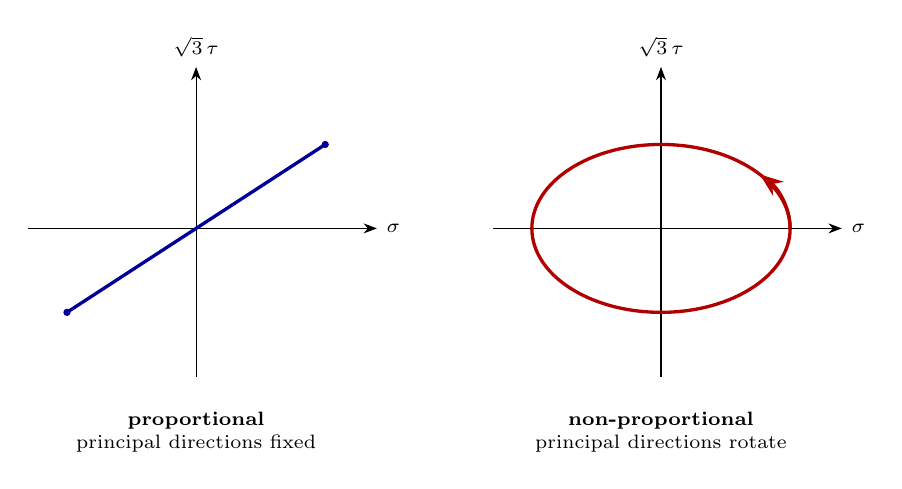
\begin{tikzpicture}[scale=0.82,>=Stealth,font=\scriptsize]
\begin{scope}
\draw[->] (-2.6,0) -- (2.8,0) node[right] {$\sigma$};
\draw[->] (0,-2.3) -- (0,2.5) node[above] {$\sqrt3\,\tau$};
\draw[very thick,blue!60!black] (-2.0,-1.3) -- (2.0,1.3);
\fill[blue!60!black] (2.0,1.3) circle (1.6pt); \fill[blue!60!black] (-2.0,-1.3) circle (1.6pt);
\node[anchor=north,align=center] at (0,-2.7) {\textbf{proportional}\\ principal directions fixed};
\end{scope}
\begin{scope}[xshift=7.2cm]
\draw[->] (-2.6,0) -- (2.8,0) node[right] {$\sigma$};
\draw[->] (0,-2.3) -- (0,2.5) node[above] {$\sqrt3\,\tau$};
\draw[very thick,red!70!black] (0,0) ellipse (2.0 and 1.3);
\draw[->,red!70!black,very thick] (2.0,0) arc (0:40:2.0 and 1.3);
\node[anchor=north,align=center] at (0,-2.7) {\textbf{non-proportional}\\ principal directions rotate};
\end{scope}
\end{tikzpicture}

\raggedright\footnotesize
Both states can have \emph{identical} von Mises amplitudes and identical static margins. Under cyclic loading the non-proportional case can have a life an order of magnitude shorter.
\end{frame}


\begin{frame}{\emph{Why} does a rotating stress state do more damage?}
\centering
\scalebox{0.82}{
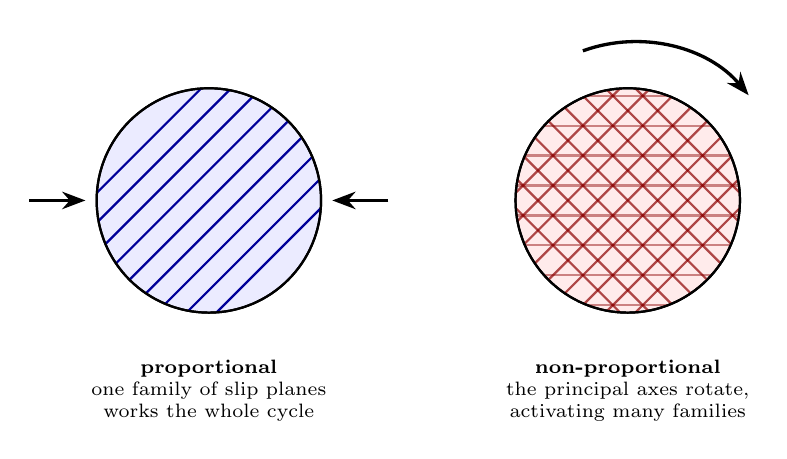
\begin{tikzpicture}[scale=0.95,>=Stealth,font=\scriptsize]
\begin{scope}
\draw[thick,fill=blue!8] (0,0) circle (1.5);
\begin{scope}\clip (0,0) circle (1.5);
\foreach \i in {-1.6,-1.2,...,1.7} \draw[blue!60!black,thick] ({\i-1.6},{-1.6}) -- ({\i+1.6},{1.6});
\end{scope}
\draw[thick] (0,0) circle (1.5);
\draw[->,very thick] (-2.4,0) -- (-1.65,0); \draw[->,very thick] (2.4,0) -- (1.65,0);
\node[anchor=north,align=center] at (0,-2.0) {\textbf{proportional}\\ one family of slip planes\\ works the whole cycle};
\end{scope}
\begin{scope}[xshift=5.6cm]
\draw[thick,fill=red!8] (0,0) circle (1.5);
\begin{scope}\clip (0,0) circle (1.5);
\foreach \i in {-1.6,-1.2,...,1.7} \draw[red!55!black,thick,opacity=0.7] ({\i-1.6},{-1.6}) -- ({\i+1.6},{1.6});
\foreach \i in {-1.6,-1.2,...,1.7} \draw[red!55!black,thick,opacity=0.7] ({\i-1.6},{1.6}) -- ({\i+1.6},{-1.6});
\foreach \i in {-1.4,-1.0,...,1.5} \draw[red!55!black,thick,opacity=0.45] (-1.6,\i) -- (1.6,\i);
\end{scope}
\draw[thick] (0,0) circle (1.5);
\draw[->,very thick] (-0.6,2.0) arc (110:40:2.0);
\node[anchor=north,align=center] at (0,-2.0) {\textbf{non-proportional}\\ the principal axes rotate,\\ activating many families};
\end{scope}
\end{tikzpicture}
}

\raggedright\footnotesize
Fatigue damage is cyclic slip on crystallographic planes. Under \alert{proportional} loading the same family of planes is worked every cycle; the material hardens on those planes and settles down. Under \alert{non-proportional} loading the principal axes sweep round, so \emph{many} families are activated in turn, none gets to settle, and the material hardens an extra 20--40\% --- with more slip activity overall, so the life goes \emph{down}, not up. \alert{The one place in this course where extra hardening is bad news.}
\end{frame}

\begin{frame}{Why static analysis does not care, but fatigue does}
\begin{columns}[T]
\column{0.48\textwidth}
\textbf{Static}
\begin{itemize}\footnotesize
  \item Evaluate von Mises at the worst instant, compare with $S_y$
  \item The path taken to get there is \alert{irrelevant}
\end{itemize}
\column{0.52\textwidth}
\textbf{Fatigue}
\begin{itemize}\footnotesize
  \item Damage accumulates by cyclic slip on particular crystallographic planes
  \item A rotating principal direction sweeps slip activity around and hardens the material an extra 20--40\%
  \item Counter-intuitively this \alert{shortens} life --- typically 2--10$\times$ for 90$^\circ$ out-of-phase loading
\end{itemize}
\end{columns}
\vspace{6pt}
\begin{alertblock}{}
The whole \emph{path} matters, not just the worst instant.
\end{alertblock}
\end{frame}

\section{Equivalent-stress methods}


\begin{frame}{Where the 3 in $3\tau^{2}$ comes from}
You met von Mises in Lecture 1 as a \emph{static} criterion:
\[
\sigma'=\sqrt{\sigma_x^{2}+3\tau_{xy}^{2}}\;\le\;\frac{S_y}{n}
\]
\begin{itemize}
  \item The factor 3 is not a fudge: it falls out of the distortion-energy derivation, and it says that \alert{shear is about $\sqrt3$ times as damaging as direct stress} for a given numerical value
  \item Equivalently, the shear yield strength is $S_{sy}=0.577\,S_y=S_y/\sqrt3$
\end{itemize}
\vspace{2pt}
\begin{block}{The step we take today}
Apply the \emph{same} formula separately to the alternating parts and to the mean parts of each component. That is all Eqs.\ (1)--(2) do --- it is von Mises used twice, not a new theory.
\end{block}
\vspace{2pt}
\footnotesize And because $S_{se}\approx0.577S_e$ for ductile metals, the Gough ellipse you will see in a moment is \emph{the same statement} written as a curve.
\end{frame}

\begin{frame}{The von Mises amplitude}
Compute the amplitude and mean of each \emph{component} separately, then combine:
\begin{align*}
\sigma'_a&=\sqrt{(K_f\sigma_a)^2+3(K_{fs}\tau_a)^2}, &
\sigma'_m&=\sqrt{(K_f\sigma_m)^2+3(K_{fs}\tau_m)^2}
\end{align*}
and feed them into any Lecture 2 mean-stress criterion. With Goodman:
\[
\frac{1}{n}=\frac{\sigma'_a}{S_e}+\frac{\sigma'_m}{S_{ut}}
\qquad\text{(\alert{DE--Goodman})}
\]
For a solid round shaft of diameter $d$ this becomes the sizing equation:
\[
\frac{1}{n}=\frac{16}{\pi d^{3}}\left\{
\frac{\big[4(K_fM_a)^{2}+3(K_{fs}T_a)^{2}\big]^{1/2}}{S_e}
+\frac{\big[4(K_fM_m)^{2}+3(K_{fs}T_m)^{2}\big]^{1/2}}{S_{ut}}\right\}
\]
\end{frame}

\begin{frame}{Two things the von Mises amplitude gets wrong}
\begin{alertblock}{1. It is positive, so it is blind to sign}
$\sigma'_m$ cannot distinguish tension from compression --- and a \emph{compressive} mean is beneficial. The repair: carry the sign of the dominant principal stress (or of the hydrostatic stress) into $\sigma'_m$, otherwise you count a benefit as damage.
\end{alertblock}
\begin{alertblock}{2. It assumes proportional loading}
Collapsing the history to amplitudes and means component by component \alert{silently discards the phase relationship}. For non-proportional loading the method is \emph{non-conservative}, sometimes badly so.
\end{alertblock}
\vspace{2pt}
\begin{block}{A practical rule for this course}
\footnotesize Loads from \emph{one} source, rising and falling together $\Rightarrow$ use it with confidence. Loads from \emph{independent} sources $\Rightarrow$ use it, but say so, and either apply a factor of 2 on life or justify the phasing from the mission.
\end{block}
\end{frame}

\begin{frame}{The Gough ellipse: bending $+$ torsion}
\begin{columns}[T]
\column{0.42\textwidth}
\[
\left(\frac{\sigma_a}{S_e}\right)^{2}+\left(\frac{\tau_a}{S_{se}}\right)^{2}=1
\]
\begin{itemize}\footnotesize
  \item $S_{se}\approx0.577\,S_e$ for ductile metals --- which makes this \alert{identical} to von Mises on amplitudes
  \item Brittle and heavily notched materials: $S_{se}/S_e$ nearer 0.8, shift the curve
  \item $n$ = the ratio in which the load line is extended to meet the curve
\end{itemize}
\column{0.58\textwidth}
\centering
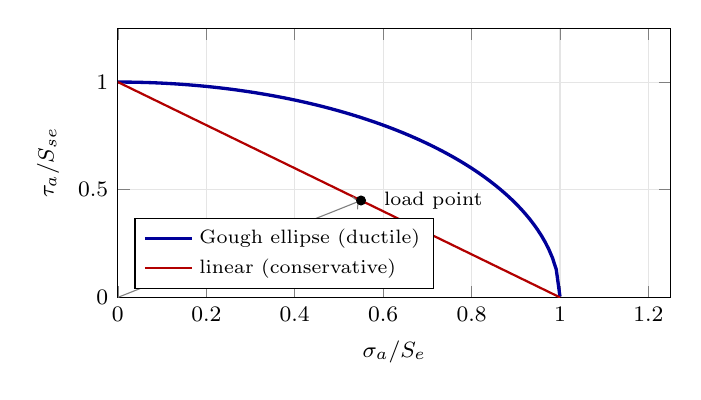
\begin{tikzpicture}
\begin{axis}[width=8.6cm,height=5.0cm,xlabel={$\sigma_a/S_e$},ylabel={$\tau_a/S_{se}$},
 xmin=0,xmax=1.25,ymin=0,ymax=1.25,grid=both,grid style={gray!20},
 label style={font=\footnotesize},tick label style={font=\footnotesize},
 legend pos=south west,legend style={font=\scriptsize},legend cell align=left]
\addplot[very thick,blue!60!black,domain=0:1,samples=120]{sqrt(1-x^2)};
\addlegendentry{Gough ellipse (ductile)}
\addplot[thick,red!70!black,domain=0:1,samples=2]{1-x};
\addlegendentry{linear (conservative)}
\addplot[only marks,mark=*,mark size=1.6pt,black] coordinates {(0.55,0.45)};
\node[font=\scriptsize,anchor=west] at (axis cs:0.58,0.45) {load point};
\draw[->,gray] (axis cs:0,0) -- (axis cs:0.55,0.45);
\end{axis}
\end{tikzpicture}
\end{columns}
\end{frame}

\begin{frame}{Critical-plane methods --- when equivalent stress fails}
Non-proportional loading defeats \emph{any} single scalar. Critical-plane methods search over candidate planes and take the worst:
\vspace{2pt}
\begin{description}\footnotesize
  \item[Findley] $\left(\tau_a+k\,\sigma_{n,\max}\right)_{\max}$ --- shear-driven with a normal-stress correction. Hard metals, long lives
  \item[Smith--Watson--Topper] $\left(\sigma_{n,\max}\,\varepsilon_{n,a}\right)_{\max}$ --- tensile-driven; materials that crack on planes of maximum normal strain
  \item[Fatemi--Socie] $\gamma_a\left(1+k\,\sigma_{n,\max}/\sigma_y\right)$ --- shear-driven with a crack-opening correction; the usual choice for non-proportional multiaxial fatigue
\end{description}
\vspace{4pt}
\begin{block}{}
These are what commercial fatigue codes run. \alert{Know they exist and when they are required.} In this course we use equivalent stress, state the proportionality assumption, and apply a knock-down when the loading is out of phase.
\end{block}
\end{frame}

\section{Counting the cycles}

\begin{frame}{Why counting is a real problem}
A measured strain-gauge record is a continuous irregular signal with peaks and valleys at every scale. The S--N curve wants an amplitude \emph{and} a count; the record supplies neither.
\vspace{4pt}
\begin{alertblock}{The question}
Is an excursion from $+240$ down to $-120$ and back to $+180$ \alert{one large cycle with a small interruption}, or \alert{two small cycles}?
\end{alertblock}
\vspace{2pt}
At $m\approx4$ in the damage law the answer changes the computed damage by an order of magnitude. This is not bookkeeping --- it is physics.
\vspace{4pt}
\begin{block}{What the material says}
\footnotesize If an excursion is interrupted and then resumed, the material closes a small hysteresis loop during the interruption and then continues along the original path \emph{as if nothing had happened}. \alert{One closed hysteresis loop is one fatigue cycle.}
\end{block}
\end{frame}


\begin{frame}{The material's answer: one closed loop is one cycle}
\begin{columns}[T]
\column{0.50\textwidth}
\centering
\scalebox{0.78}{
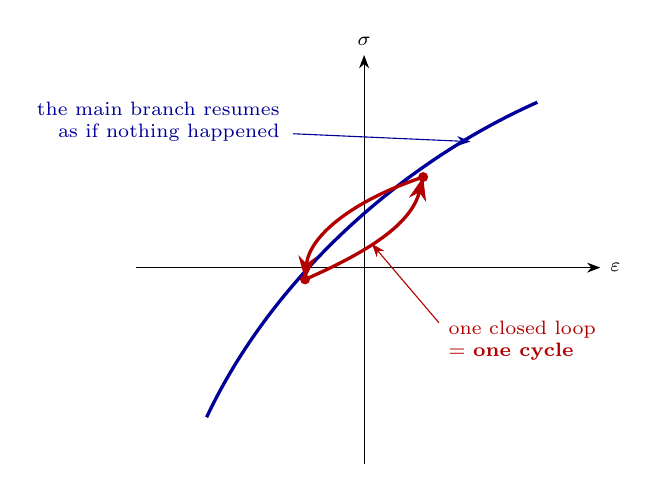
\begin{tikzpicture}[scale=1.0,>=Stealth,font=\scriptsize]
\draw[->] (-2.9,0) -- (3.0,0) node[right] {$\varepsilon$};
\draw[->] (0,-2.5) -- (0,2.7) node[above] {$\sigma$};
% main loading branch up
\draw[very thick,blue!60!black] (-2.0,-1.9) .. controls (-1.2,-0.2) and (0.4,1.3) .. (2.2,2.1);
% small interruption loop, drawn wide enough to read
\draw[very thick,red!70!black,->] (0.75,1.15) .. controls (-0.15,0.85) and (-0.7,0.4) .. (-0.75,-0.15);
\draw[very thick,red!70!black,->] (-0.75,-0.15) .. controls (0.05,0.2) and (0.6,0.55) .. (0.75,1.15);
\fill[red!70!black] (0.75,1.15) circle (1.8pt);
\fill[red!70!black] (-0.75,-0.15) circle (1.8pt);
\node[red!70!black,anchor=north west,align=left] at (0.95,-0.55) {one closed loop\\ $=$ \textbf{one cycle}};
\draw[->,red!70!black] (0.95,-0.7) -- (0.1,0.3);
\node[blue!60!black,anchor=east,align=right] at (-0.95,1.85) {the main branch resumes\\ as if nothing happened};
\draw[->,blue!60!black] (-0.9,1.7) -- (1.35,1.6);
\end{tikzpicture}
}
\column{0.50\textwidth}
\footnotesize
Plot stress against \emph{strain}, not against time:
\begin{itemize}
  \item A large excursion traces a long branch
  \item An interruption part-way up traces a \alert{small closed loop} and returns to the branch
  \item The material then carries on up the original branch \alert{as if the interruption had never happened} --- this is the \emph{memory} effect
\end{itemize}
\vspace{2pt}
So ``one big cycle or two small ones?'' has a physical answer: \alert{one big cycle \emph{and} one small one}.
\end{columns}
\vspace{2pt}
\begin{alertblock}{}
\footnotesize Rainflow counting is just the bookkeeping that finds these loops in a time history. Everything in the algorithm follows from this picture.
\end{alertblock}
\end{frame}

\begin{frame}{Rainflow counting (ASTM E1049)}
The algorithm that extracts exactly those closed loops --- the only counting method consistent with the material's memory, and universal in practice.
\vspace{4pt}
\begin{block}{The three-point rule}
Work along the reversals, keeping a stack. Examine the last three $S_1,S_2,S_3$; let $Y=|S_2-S_1|$ and $X=|S_3-S_2|$:
\begin{itemize}\footnotesize
  \item \alert{$X\ge Y$}: the range $Y$ closes. \emph{Count one full cycle of range $Y$, mean $(S_1+S_2)/2$}; discard $S_1,S_2$; repeat the test
  \item \alert{$X<Y$}: nothing closes. Read the next reversal and repeat
\end{itemize}
What remains at the end is the \textbf{residue}, counted as \emph{half} cycles.
\end{block}
\vspace{2pt}
\footnotesize For a repeating block, join the residue head to tail and re-count so nothing is lost between blocks. Level-crossing, peak and range counting are its cruder ancestors --- do not use them.
\end{frame}

\begin{frame}{What rainflow found, drawn on the history}
\centering

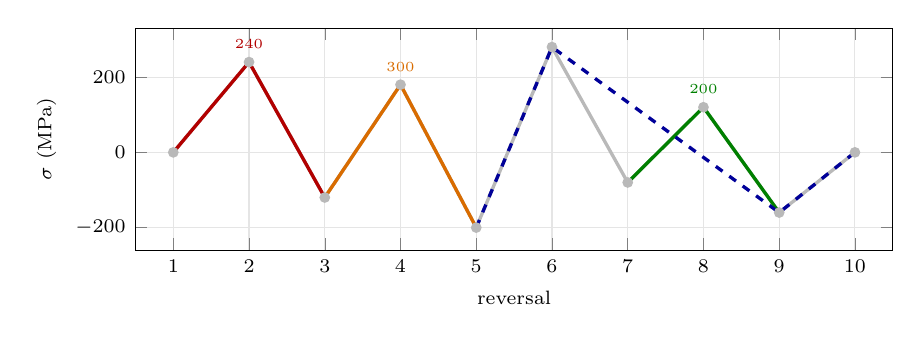
\begin{tikzpicture}[scale=1.0,>=Stealth,font=\scriptsize]
\begin{axis}[width=11.2cm,height=4.4cm,xlabel={reversal},ylabel={$\sigma$ (MPa)},
  xmin=0.5,xmax=10.5,ymin=-260,ymax=330,grid=both,grid style={gray!20},
  xtick={1,2,...,10},
  label style={font=\scriptsize},tick label style={font=\scriptsize}]
\addplot[very thick,gray!55,mark=*,mark size=1.3pt] coordinates
 {(1,0)(2,240)(3,-120)(4,180)(5,-200)(6,280)(7,-80)(8,120)(9,-160)(10,0)};
% counted cycles highlighted
\addplot[very thick,red!70!black] coordinates {(1,0)(2,240)(3,-120)};
\addplot[very thick,orange!85!black] coordinates {(3,-120)(4,180)(5,-200)};
\addplot[very thick,green!50!black] coordinates {(7,-80)(8,120)(9,-160)};
\node[font=\tiny,red!70!black,anchor=south] at (axis cs:2,250) {240};
\node[font=\tiny,orange!85!black,anchor=south] at (axis cs:4,190) {300};
\node[font=\tiny,green!50!black,anchor=south] at (axis cs:8,130) {200};
% residue
\addplot[very thick,blue!60!black,dashed] coordinates {(5,-200)(6,280)(9,-160)(10,0)};

\end{axis}
\end{tikzpicture}

\vspace{-2pt}

\raggedright\footnotesize
The three coloured excursions are the cycles that \alert{closed} inside the block: ranges \textcolor{red!70!black}{\textbf{240}}, \textcolor{orange!85!black}{\textbf{300}} and \textcolor{green!50!black}{\textbf{200}}. The dashed path is the \alert{residue} --- the large excursions that never closed, counted as half cycles of range \textbf{480}, \textbf{440} and \textbf{160}.
\vspace{2pt}

\begin{alertblock}{}
\footnotesize Notice that the three \emph{largest} ranges are all in the residue. That is typical, and it is why residue handling matters: discard it and you throw away most of the damage.
\end{alertblock}
\end{frame}

\begin{frame}{Example 4.3 --- counting by hand}
\footnotesize
$0,\;+240,\;-120,\;+180,\;-200,\;+280,\;-80,\;+120,\;-160,\;0$ \si{MPa}
\vspace{2pt}
\centering
\begin{tabular}{@{}llll@{}}
\toprule
Stack (last three) & $Y$ & $X$ & Action \\
\midrule
$0,\,240,\,-120$ & 240 & 360 & $X\ge Y$: count \textbf{240}, mean $+120$; discard $0,240$ \\
$-120,\,180,\,-200$ & 300 & 380 & $X\ge Y$: count \textbf{300}, mean $+30$; discard $-120,180$ \\
$-200,\,280,\,-80$ & 480 & 360 & $X<Y$: read on \\
$280,\,-80,\,120$ & 360 & 200 & $X<Y$: read on \\
$-80,\,120,\,-160$ & 200 & 280 & $X\ge Y$: count \textbf{200}, mean $+20$; discard $-80,120$ \\
$-200,\,280,\,-160$ & 480 & 440 & $X<Y$: read on \\
$280,\,-160,\,0$ & 440 & 160 & $X<Y$: end of block \\
\bottomrule
\end{tabular}
\vspace{4pt}

\raggedright
Residue $-200,\,280,\,-160,\,0$ $\Rightarrow$ half cycles of range \textbf{480} (mean $+40$), \textbf{440} (mean $+60$), \textbf{160} (mean $-80$).
\end{frame}

\section{Damage over a spectrum}


\begin{frame}{Step 2: turning a counted cycle into an equivalent amplitude}
\begin{columns}[T]
\column{0.56\textwidth}
\centering

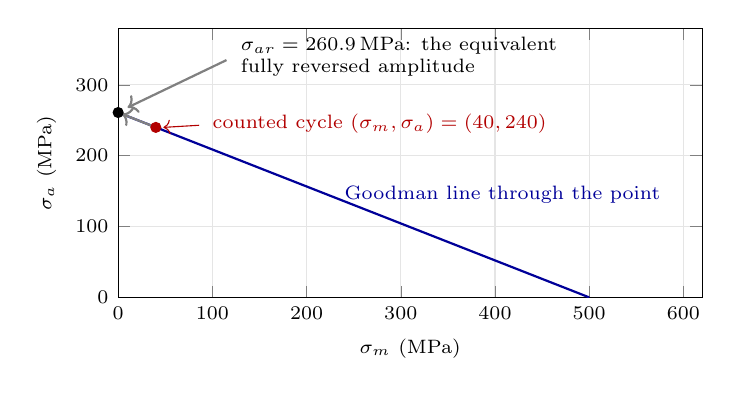
\begin{tikzpicture}
\begin{axis}[width=9.0cm,height=5.0cm,xlabel={$\sigma_m$ (MPa)},ylabel={$\sigma_a$ (MPa)},
 xmin=0,xmax=620,ymin=0,ymax=380,grid=both,grid style={gray!20},
 label style={font=\scriptsize},tick label style={font=\scriptsize}]
\addplot[thick,blue!60!black,domain=0:500,samples=2]{261*(1-x/500)};
\node[font=\scriptsize,blue!60!black,anchor=west] at (axis cs:230,145) {Goodman line through the point};
\addplot[only marks,mark=*,mark size=1.8pt,red!70!black] coordinates {(40,240)};
\node[font=\scriptsize,red!70!black,anchor=west] at (axis cs:90,245) {counted cycle $(\sigma_m,\sigma_a)=(40,240)$};
\draw[->,red!70!black] (axis cs:86,243) -- (axis cs:48,240);
\addplot[only marks,mark=*,mark size=1.8pt,black] coordinates {(0,261)};
\node[font=\scriptsize,anchor=west,align=left] at (axis cs:120,340) {$\sigma_{ar}=\SI{260.9}{MPa}$: the equivalent\\ fully reversed amplitude};
\draw[->,thick,gray] (axis cs:115,335) -- (axis cs:10,268);
\draw[->,thick,gray] (axis cs:40,240) -- (axis cs:4,259);
\end{axis}
\end{tikzpicture}

\column{0.44\textwidth}
\footnotesize
Each counted cycle arrives as a pair $(\sigma_a,\sigma_m)$. The S--N curve only knows about \emph{fully reversed} loading, so we must ask:
\vspace{2pt}

\alert{what fully reversed amplitude would do the same damage?}
\vspace{4pt}

Draw the Goodman line through the point to the $\sigma_m$ axis at $S_{ut}$; where it cuts the $\sigma_a$ axis is $\sigma_{ar}$:
\[
\sigma_{ar}=\frac{\sigma_a}{1-\sigma_m/S_{ut}}
\]
Here $240/(1-40/500)=\SI{260.9}{MPa}$ --- a tensile mean has made the cycle \alert{more} damaging.
\end{columns}
\end{frame}

\begin{frame}{Miner on the counted spectrum}
Correct each cycle to an equivalent fully reversed amplitude, then sum:
\[
\sigma_{ar}=\frac{\sigma_a}{1-\sigma_m/S_{ut}}\ (\sigma_m>0),\qquad
D=\sum_i\frac{n_i}{N_i}
\]
\centering\footnotesize
\begin{tabular}{@{}rrrrrrrl@{}}
\toprule
range & mean & $n_i$ & $\sigma_a$ & $\sigma_{ar}$ & $N_i$ & $n_i/N_i$ & share \\
\midrule
480 &  40 & 0.5 & 240 & 260.9 & $3.33\times10^{5}$ & $1.50\times10^{-6}$ & \alert{56.6\%} \\
440 &  60 & 0.5 & 220 & 250.0 & $4.75\times10^{5}$ & $1.05\times10^{-6}$ & \alert{39.7\%} \\
300 &  30 & 1.0 & 150 & 159.6 & $2.00\times10^{7}$ & $4.99\times10^{-8}$ & 1.9\% \\
240 & 120 & 1.0 & 120 & 157.9 & $2.19\times10^{7}$ & $4.57\times10^{-8}$ & 1.7\% \\
200 &  20 & 1.0 & 100 & 104.2 & $7.01\times10^{8}$ & $1.43\times10^{-9}$ & 0.1\% \\
160 & $-80$ & 0.5 & 80 & 80.0 & $6.32\times10^{9}$ & $7.91\times10^{-11}$ & 0.0\% \\
\bottomrule
\end{tabular}
\vspace{3pt}

\raggedright\normalsize
$D=2.65\times10^{-6}$ per block $\Rightarrow$ $3.78\times10^{5}$ blocks; with a scatter factor of 4, $9.4\times10^{4}$.
\end{frame}

\begin{frame}{Read the last column}
\begin{alertblock}{Three reversals out of nine do 96\% of the damage}
The two largest half-cycles carry almost everything. The three smallest cycles together do 0.1\%.
\end{alertblock}
\vspace{4pt}
This is the shape of \emph{every} spectrum calculation you will do, and it has two consequences:
\begin{itemize}
  \item \alert{Truncating the small cycles changes nothing} --- which is why spectra are routinely truncated at the low end to save computation
  \item \alert{Any design change that clips the largest ranges pays enormously} --- and truncating the \emph{high} end is a serious error
\end{itemize}
\end{frame}

\begin{frame}{What Miner ignores}
\begin{columns}[T]
\column{0.5\textwidth}
\begin{itemize}\footnotesize
  \item \textbf{Sequence.} High--low is more damaging than low--high: the large cycles initiate a crack the small ones then grow. Miner is order-blind
  \item \textbf{Cycles below $S_e$.} Strict Miner discards them --- but once a crack exists, small cycles \emph{do} grow it
\end{itemize}
\column{0.5\textwidth}
\begin{itemize}\footnotesize
  \item \textbf{Interaction.} Overloads retard, underloads accelerate; neither is in the sum
  \item \textbf{Scatter.} Test data fail anywhere from $D=0.3$ to $D=3$
\end{itemize}
\end{columns}
\vspace{4pt}
\begin{block}{The Haibach correction}
\footnotesize Continue the S--N line beyond the knee with a shallower slope $(2m-1)$ instead of truncating. The usual compromise.
\end{block}
\begin{alertblock}{}
The practical answer is not a better damage rule --- it is a \alert{scatter factor} on the computed life, backed by a full-scale test. Which is exactly what certification requires.
\end{alertblock}
\end{frame}

\section{The aircraft spectrum}

\begin{frame}{Where a design spectrum comes from}
\footnotesize
\begin{tabular}{@{}llp{7.0cm}@{}}
\toprule
Source & Frequency & Character \\
\midrule
Ground--air--ground & 1 per flight & largest single range; ground taxi load to 1\,g airborne and back. \alert{Usually the dominant contributor} \\
Pressurisation & 1 per flight & zero to full $\Delta p$; sizes fuselage lap joints \\
Gust & many per hour & from statistical exceedance curves; depends on altitude, speed, terrain \\
Manoeuvre & few per flight & from the mission profile and the $V$--$n$ diagram \\
Taxi, landing, braking & few per flight & high local loads; often the gear's dominant source \\
Buffet, vibration & continuous & engine, propeller or rotor order; low amplitude, enormous counts \\
\bottomrule
\end{tabular}
\vspace{4pt}

\normalsize
Assembled into a \alert{flight-by-flight sequence}: each flight built from its own phases, and the flights ordered to represent the real mix of sectors. That sequence --- not a histogram --- is the input to the analysis \emph{and} to the full-scale test, precisely because sequence effects exist even though Miner cannot see them.
\end{frame}

\begin{frame}{The usage spectrum is a design input}
\begin{alertblock}{Two aircraft of the same type, different missions, different damage rates}
An island-hopper flies five times as many pressurisation cycles per flight \emph{hour} as a long-haul aircraft of the same type. A trainer flies far more manoeuvre cycles than a tourer.
\end{alertblock}
\vspace{4pt}
\begin{itemize}
  \item If the usage changes, \alert{the fatigue substantiation must be revisited}
  \item This is the lesson behind the ageing-aircraft programmes
  \item And it is why a maintenance programme is written against flight \alert{cycles}, not hours
\end{itemize}
\vspace{4pt}
\footnotesize Aloha 243: 89\,680 cycles against a 75\,000-cycle design goal, on 30-minute island sectors in salt air.
\end{frame}

\section{Scatter}

\begin{frame}{Scatter and the design S--N curve}
At a given stress amplitude, fatigue lives routinely span a factor of ten --- and the scatter \emph{grows} as the stress falls. ASTM E739 sets out the fit and its confidence bands.
\vspace{4pt}
\begin{itemize}
  \item \alert{The design curve is not the mean curve.} It is a lower bound at a stated survival probability --- commonly mean minus three standard deviations of $\log N$, or a $95/95$ tolerance bound. The fatigue analogue of A- and B-basis
  \item \alert{Regress $\log N$ on $\log S$, not the reverse.} Stress is the controlled variable, life is the random one. Fitting the wrong way round gives a visibly different --- and non-conservative --- line
\end{itemize}
\vspace{4pt}
\begin{block}{What you will actually meet in MMPDS}
\footnotesize $S_{eq}=S_{\max}(1-R)^{p}$, which collapses several $R$ ratios onto one curve with $p\approx0.4$--$0.6$ fitted to the data. A third way of handling mean stress, alongside Goodman and the rest.
\end{block}
\end{frame}

\section{Worked examples}

\begin{frame}{Example 4.1 --- Shaft in combined bending and torsion}
4340, $d=\SI{45}{mm}$, $S_{ut}=\SI{1240}{MPa}$, $S_e=\SI{300}{MPa}$; $M_a=\SI{620}{N.m}$ rotating, $T_m=\SI{480}{N.m}$ steady; $K_f=1.7$, $K_{fs}=1.4$
\vspace{-2pt}
\begin{align*}
Z&=\pi d^3/32=\SI{8946}{mm^3}, &
\sigma_a&=\frac{620\times10^{3}}{8946}=\SI{69.3}{MPa}, &
\tau_m&=\frac{480\times10^{3}}{2Z}=\SI{26.8}{MPa}\\[2pt]
\sigma'_a&=1.7\times69.3=\SI{117.8}{MPa}, &
\sigma'_m&=\sqrt{3}\times1.4\times26.8=\SI{65.0}{MPa} & &\\[2pt]
\frac{1}{n}&=\frac{117.8}{300}+\frac{65.0}{1240}&&=0.3927+0.0524 &&\Rightarrow\ n=\mathbf{2.25}
\end{align*}
\begin{alertblock}{Two observations}
\footnotesize The alternating bending carries \alert{88\%} of the damage term even though the torque is of comparable magnitude --- because the torque is \emph{steady} and enters only through the much larger $S_{ut}$. And $K_f=1.7$ alone consumes a factor of 1.7 on the dominant term: \alert{the fillet radius is worth more than any material substitution}.
\end{alertblock}
\end{frame}

\begin{frame}{Example 4.2 --- Why phasing matters}
Landing-gear axle: $\sigma_a=\SI{180}{MPa}$ from vertical load, $\tau_a=\SI{90}{MPa}$ from braking. $S_e=\SI{320}{MPa}$, $S_{se}=\SI{185}{MPa}$.
\[
\left(\frac{180}{320}\right)^{2}+\left(\frac{90}{185}\right)^{2}=0.316+0.237=0.553<1
\quad\Rightarrow\quad n=1/\sqrt{0.553}=1.34
\]
\begin{alertblock}{But the loads are not proportional}
Braking happens at touchdown with a particular vertical load; the two histories have no fixed ratio. For 90$^\circ$ out-of-phase bending and torsion, test data show \alert{life reductions of 2 to 10 times}.
\end{alertblock}
\vspace{2pt}
\footnotesize $n=1.34$ on stress is $1.34^{4}=3.2$ on life at $m=4$ --- which the non-proportionality can erase entirely.

\textbf{What to do:} state the assumption, apply a knock-down on life, and for a critical part use a critical-plane method or test it. \alert{What you must not do} is report $n=1.34$ without saying it assumed proportional loading.
\end{frame}

\section{Design implications}

\begin{frame}{Levers, in order of effectiveness}
\begin{enumerate}
  \item \alert{Clip the peaks of the spectrum.} At $m\approx4$--7 the few largest cycles carry almost all the damage. Load alleviation, a softer suspension, a lower limit manoeuvre factor, a gust-alleviation system --- all buy more than any material change
  \item \alert{Remove the notch.} In Example 4.1 the fillet consumed a factor of 1.7 directly on the dominant term
  \item \alert{Make the loading proportional if you can.} Route two independent loads through separate members rather than superimposing them on one
  \item \alert{Convert a damaging mean into a benign one.} Preload, shot peening, cold expansion
  \item \emph{Only then}: raise $S_e$ by material or treatment
\end{enumerate}
\end{frame}

\section{For next time}

\begin{frame}{For next time}
\begin{itemize}
  \item Shigley \S\S6.14--6.17 and Ch.\ 7 (shafts); Dowling Ch.\ 10 (variable amplitude) and Ch.\ 12 (multiaxial)
  \item ASTM E1049 (cycle counting) and E739 (statistical analysis of fatigue data)
  \item Self-study problems 1--6 in the notes --- problem 4 asks you to implement rainflow counting in Python, including residue handling
  \item Next: \alert{thread standards, power screws and thread strength} --- the first of the joints block, and the mechanics behind the callouts you learned to read in Lecture 1
\end{itemize}
\end{frame}

\end{document}
